\section{System Design}
\label{sec:method}

\subsection{Overview}

Deep Researcher Agent operates as a continuous loop over three phases (Algorithm~\ref{alg:loop}). Each cycle takes the current project brief and memory log as input, produces an experiment plan, executes it, monitors to completion, analyzes results, and updates memory before beginning the next cycle. The overall architecture is shown in Figure~\ref{fig:architecture}.

\begin{figure*}[t]
\centering
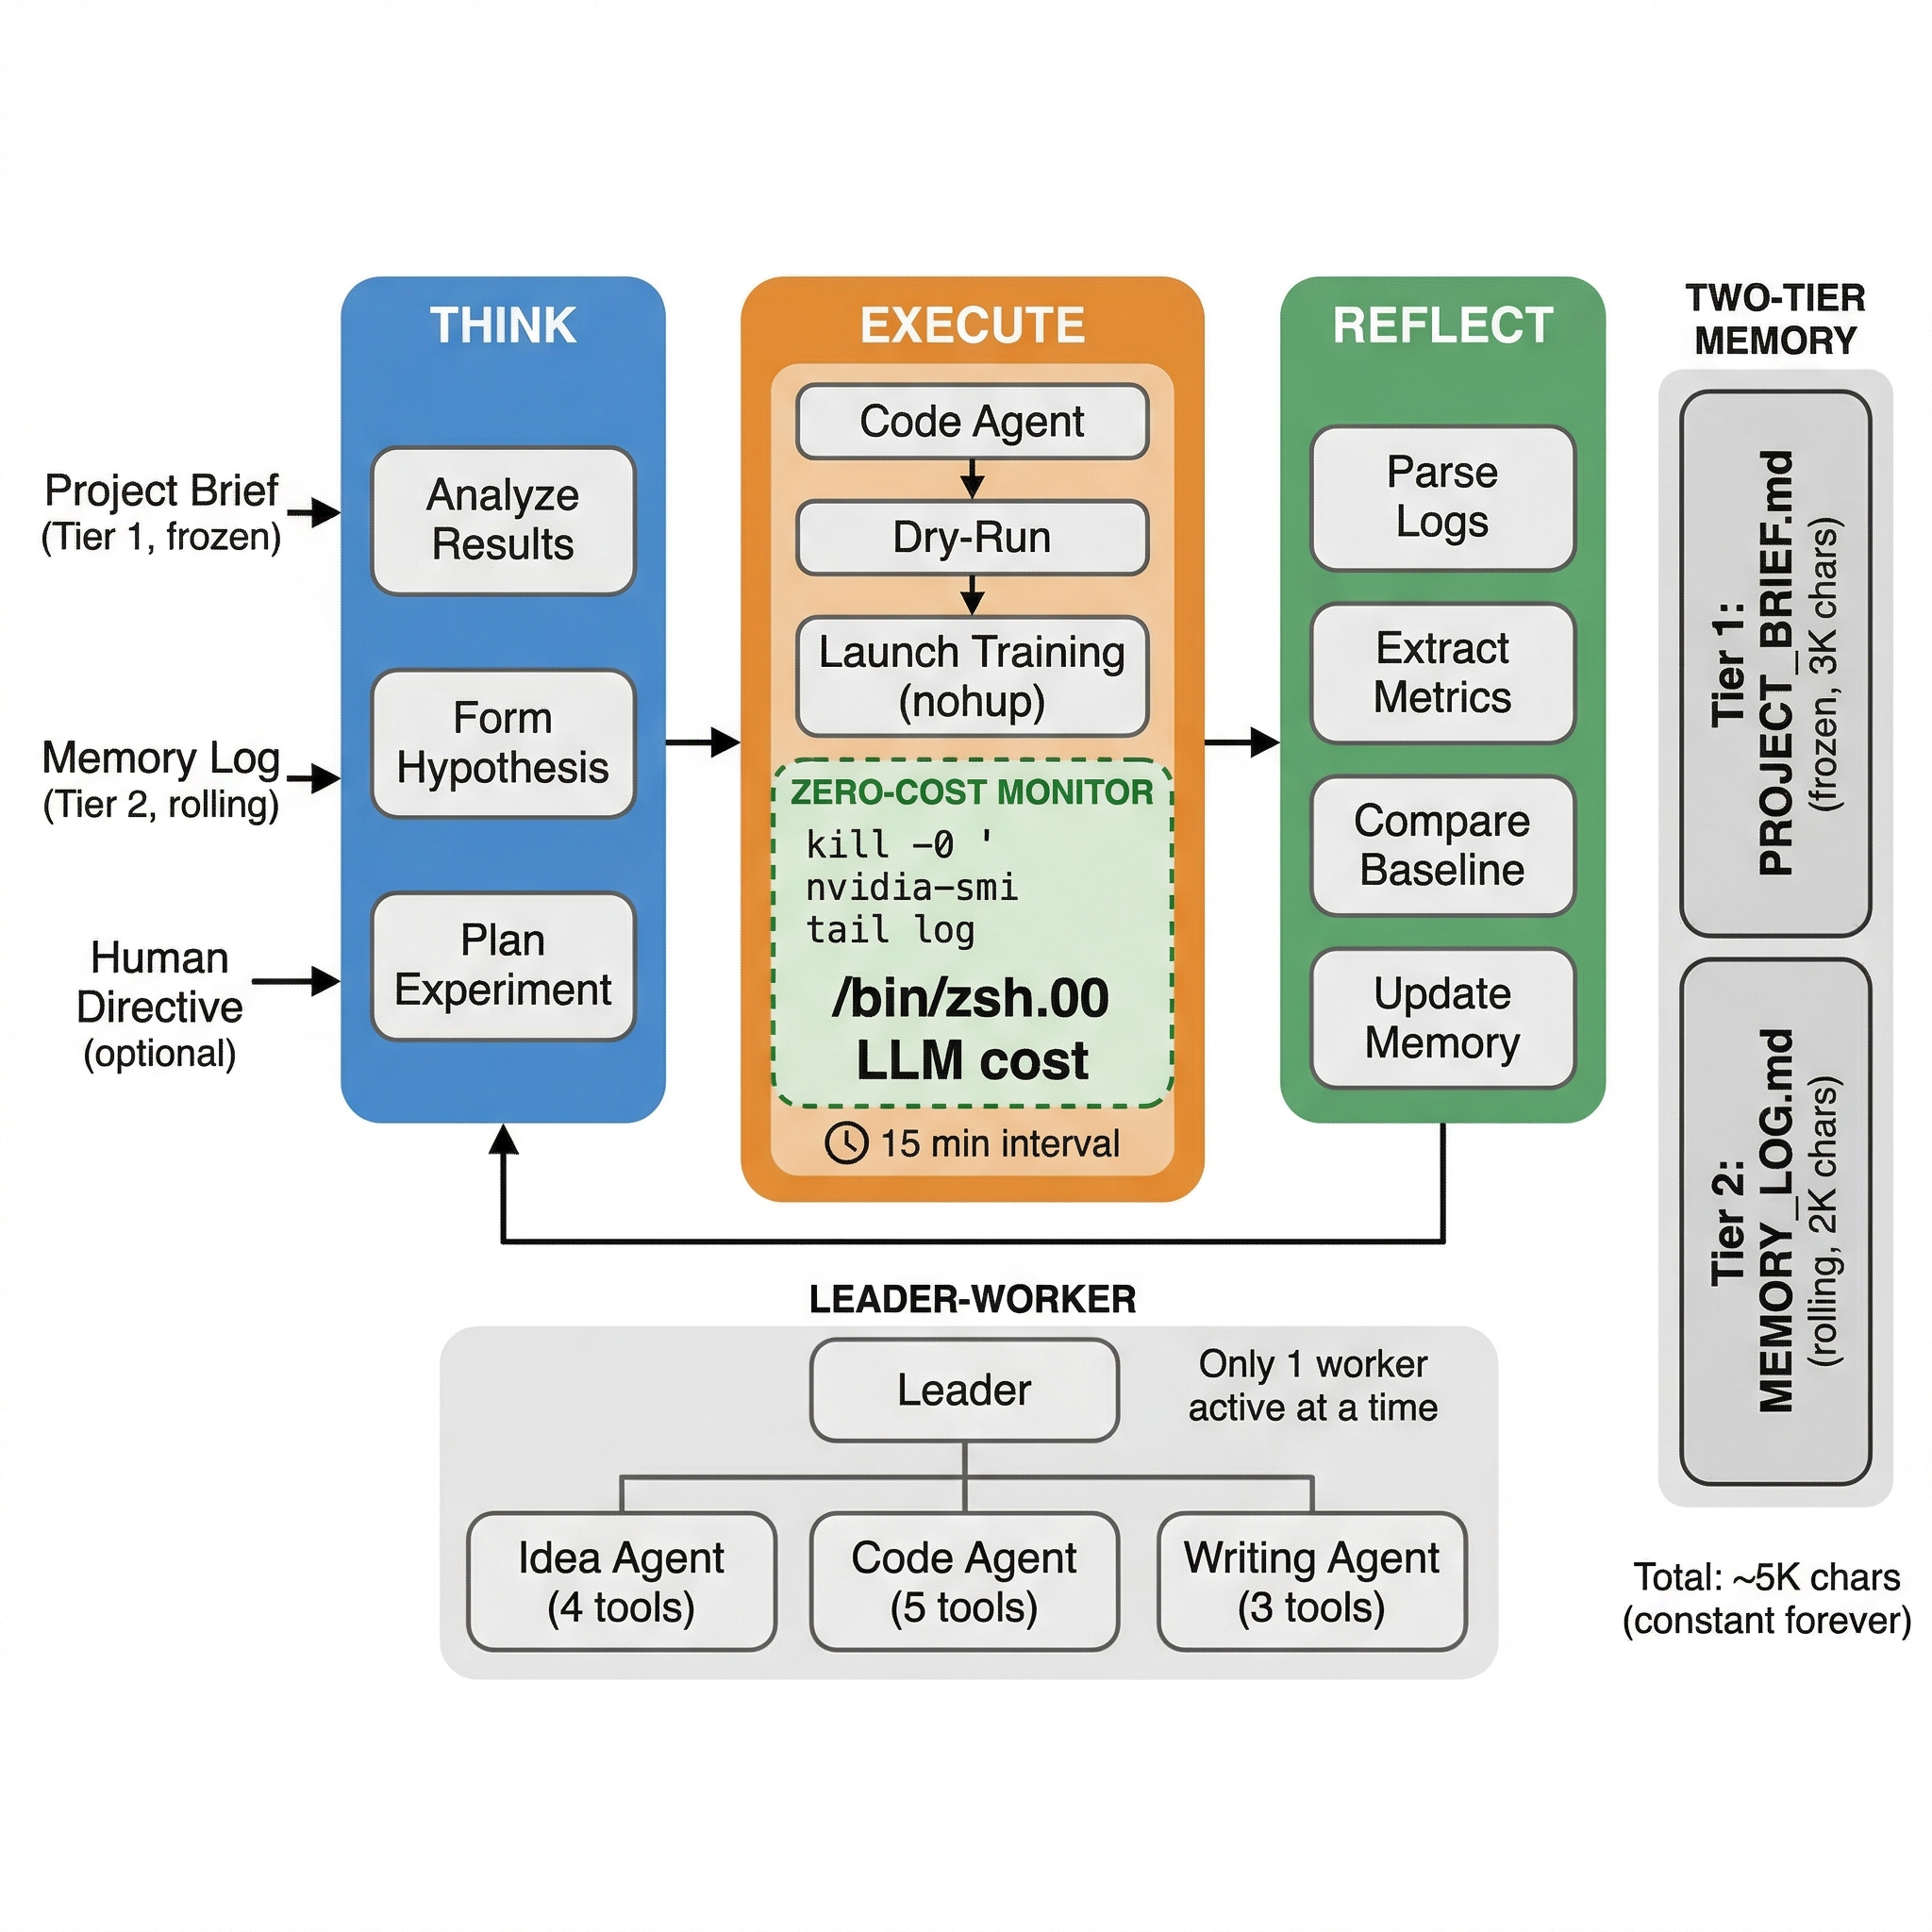
\includegraphics[width=0.95\textwidth]{figures/architecture.png}
\caption{\textbf{Overview of Deep Researcher Agent.} The system operates as a continuous \textsc{Think}$\rightarrow$\textsc{Execute}$\rightarrow$\textsc{Reflect} loop. During the \textsc{Execute} phase, training is monitored at \textbf{zero LLM cost} --- only OS-level process checks and log file reads are performed. The Two-Tier Memory system maintains a constant size ($\sim$5K chars) regardless of how long the agent runs.}
\label{fig:architecture}
\end{figure*}

\begin{algorithm}[t]
\caption{Deep Researcher Agent Main Loop}
\label{alg:loop}
\begin{algorithmic}[1]
\REQUIRE Project brief $B$, initial memory $M_0$
\STATE $t \leftarrow 0$
\WHILE{not terminated}
    \STATE $t \leftarrow t + 1$
    \STATE $d \leftarrow \textsc{ConsumeDirective}()$ \COMMENT{Human override}
    \STATE \textcolor{thinkcolor}{$plan_t \leftarrow \textsc{Think}(B, M_{t-1}, d)$} \COMMENT{LLM active}
    \IF{$plan_t.\text{action} = \text{``wait''}$}
        \STATE \textsc{SmartCooldown}()
        \STATE \textbf{continue}
    \ENDIF
    \STATE \textcolor{execcolor}{$result_t \leftarrow \textsc{Execute}(plan_t)$} \COMMENT{LLM $\rightarrow$ training}
    \IF{$result_t.\text{launched}$}
        \STATE $logs_t \leftarrow \textsc{Monitor}(result_t.\text{pid})$ \COMMENT{\textbf{Zero cost}}
    \ENDIF
    \STATE \textcolor{reflectcolor}{$M_t \leftarrow \textsc{Reflect}(B, M_{t-1}, result_t, logs_t)$} \COMMENT{LLM active}
\ENDWHILE
\end{algorithmic}
\end{algorithm}

\subsection{Zero-Cost Monitoring}
\label{sec:zero-cost}

The central insight of our design is that during GPU training --- which constitutes 90--99\% of wall-clock time in a typical experiment cycle --- the LLM has nothing useful to contribute. The training process follows a predetermined schedule, and intermediate results (loss curves, validation metrics) are written to log files automatically by the training script.

We exploit this observation by implementing a monitoring phase that makes \textit{zero} LLM API calls. Instead, three lightweight OS-level checks are performed at configurable intervals (default: 15 minutes):

\begin{enumerate}[nosep]
    \item \textbf{Process liveness}: \texttt{kill -0 \$PID} checks whether the training process is still running. This is a single syscall with negligible cost.
    \item \textbf{GPU utilization}: \texttt{nvidia-smi} confirms GPU activity and rules out silent crashes where the process exists but is no longer utilizing the GPU.
    \item \textbf{Log tail}: Reading the last 50 lines of the training log provides the latest metrics for local logging without invoking the LLM.
\end{enumerate}

The LLM is only invoked when the training process terminates (detected by a non-zero return from \texttt{kill -0}), at which point the accumulated log tail is passed to the \textsc{Reflect} phase for analysis.

\paragraph{Cost Analysis.} Consider a 24-hour cycle where training takes 8 hours. A conventional agent polling the LLM every 5 minutes would make $8 \times 60 / 5 = 96$ API calls during training alone, each consuming $\sim$2K tokens (system prompt + context + response), totaling $\sim$192K tokens or approximately \$0.50 for the monitoring phase alone. Our approach reduces the monitoring cost to exactly \$0.00, with LLM costs limited to the \textsc{Think} ($\sim$\$0.05) and \textsc{Reflect} ($\sim$\$0.03) phases.

\subsection{Two-Tier Constant-Size Memory}
\label{sec:memory}

Long-running LLM agents face a fundamental problem: accumulated context grows without bound, leading to (a) degraded LLM performance as context length increases, (b) escalating API costs proportional to context size, and (c) eventual context window overflow.

We address this with a two-tier memory system bounded at $\sim$5,000 characters ($\sim$1,500 tokens), maintained constant regardless of runtime duration:

\paragraph{Tier 1: Project Brief ($B$).} A human-authored, frozen document describing the research goal, codebase structure, constraints, and success criteria. Maximum size: 3,000 characters. The agent cannot modify this tier, ensuring the research direction remains stable.

\paragraph{Tier 2: Memory Log ($M$).} An agent-maintained rolling log with two sections:
\begin{itemize}[nosep]
    \item \textbf{Key Results}: Milestone entries recording significant experimental outcomes (e.g., ``Exp003: ViT-B/16, lr=3e-4 + cosine, acc=77.9\% --- new best!''). Auto-compacted: when the section exceeds 1,200 characters, the oldest entry is removed.
    \item \textbf{Recent Decisions}: A log of the agent's reasoning for each decision. Auto-compacted: only the most recent 15 entries are retained, regardless of total character count.
\end{itemize}

The total memory size is bounded by:
\begin{equation}
    |M_t| \leq |B|_{\max} + |L|_{\max} = 3000 + 2000 = 5000 \text{ chars}, \quad \forall t
\end{equation}
where $|B|_{\max}$ and $|L|_{\max}$ are the character caps for the brief and log, respectively. This guarantee holds whether the agent has run for 1 day or 6 months.

The compaction is lossy by design --- the agent retains the most valuable information (recent decisions and best results) while discarding routine entries. This mirrors how human researchers maintain a mental model: remembering key milestones and recent context while forgetting routine details.

\subsection{Leader-Worker Architecture with Minimal Tool Sets}
\label{sec:agents}

Our multi-agent system uses a Leader-Worker pattern where the Leader agent makes strategic decisions and dispatches tasks to specialized Worker agents.

\paragraph{Leader Agent.} The central decision-maker that maintains a persistent conversation \textit{within} each cycle for coherent multi-step reasoning. Importantly, the conversation history is \textit{reset between cycles} to prevent unbounded growth. Tools: \texttt{log\_memory}, \texttt{write\_file}, \texttt{read\_file} (3 tools).

\paragraph{Worker Agents.} Three specialized workers, each with a minimal tool set:
\begin{itemize}[nosep]
    \item \textbf{Idea Agent}: Literature search and hypothesis formation. Tools: \texttt{search\_papers}, \texttt{get\_paper}, \texttt{write\_file}, \texttt{read\_file} (4 tools).
    \item \textbf{Code Agent}: Experiment implementation and execution. Tools: \texttt{run\_shell}, \texttt{launch\_experiment}, \texttt{write\_file}, \texttt{read\_file}, \texttt{list\_files} (5 tools).
    \item \textbf{Writing Agent}: Report and analysis generation. Tools: \texttt{write\_file}, \texttt{read\_file}, \texttt{list\_files} (3 tools).
\end{itemize}

Only one worker runs at a time; others are completely idle at zero token cost. The Leader dispatches at most 3 worker tasks per cycle.

\paragraph{Why Minimal Tool Sets Matter.} Each tool definition adds approximately 200 tokens to every API call (name, description, parameter schema). A typical agent framework provides 15+ tools to every agent, adding $\sim$3,000 tokens of overhead per call. Our approach averages 4 tools per agent ($\sim$800 tokens), a 73\% reduction. Over 100 API calls per day, this saves $\sim$220K tokens, translating to meaningful cost savings and faster response times.

\subsection{Safety Mechanisms}
\label{sec:safety}

\paragraph{Mandatory Dry-Run.} Before any real training launch, the Code Agent must execute a short dry-run (typically 2 forward-backward steps) to verify that the code runs without errors. This catches configuration mistakes, missing imports, and tensor shape mismatches before committing GPU hours.

\paragraph{Protected Files.} Critical state files (\texttt{state.json}, \texttt{MEMORY\_LOG.md}, \texttt{PROJECT\_BRIEF.md}) cannot be overwritten by worker agents, preventing accidental corruption of the agent's memory or configuration.

\paragraph{Human Override.} Three intervention mechanisms are provided: (1) a \texttt{HUMAN\_DIRECTIVE.md} file consumed at the start of each cycle with highest priority, (2) a command-line \texttt{--directive} flag for one-time instructions, and (3) direct modification of \texttt{MEMORY\_LOG.md} for permanent behavioral changes.

\paragraph{Anti-Burn Protection.} If consecutive cycles produce no meaningful output (e.g., repeated errors or empty results), the cooldown interval is exponentially increased (up to 30 minutes) to prevent wasteful token consumption.
